%!TEX platex=1
\documentclass[11pt,xcolor=dvipsnames,table,dvipdfmx]{beamer}
\usepackage{amsmath, amssymb}
\usepackage{latexsym}
\usepackage{ascmac}
\usepackage{bm}

%Beamer$B$N@_Dj(B
\usetheme{Boadilla}
%Beamer$B%U%)%s%H@_Dj(B
\usepackage{txfonts} % TX$B%U%)%s%H(B
\usepackage[deluxe]{otf} % $BF|K\8lB?%&%'%$%H2=(B
\renewcommand{\familydefault}{\sfdefault}  % $B1QJ8$r%5%s%;%j%UBN$K(B
\renewcommand{\kanjifamilydefault}{\gtdefault}  % $BF|K\8l$r%4%7%C%/BN$K(B
\usefonttheme{professionalfonts}
\setbeamerfont{alerted text}{series=\bfseries} % Alert$B$rB@;z(B
\setbeamerfont{section in toc}{series=\mdseries} % $BL\<!$OB@;z$K$7$J$$(B
\setbeamerfont{frametitle}{size=\Large} % $B%U%l!<%`%?%$%H%kJ8;z%5%$%:(B
\setbeamerfont{title}{size=\LARGE} % $B%?%$%H%kJ8;z%5%$%:(B
\setbeamerfont{date}{size=\small}  % $BF|IUJ8;z%5%$%:(B

%Beamer$B?'@_Dj(B
\definecolor{UniBlue}{RGB}{0,150,200} 
\definecolor{AlertOrange}{RGB}{255,76,0}
\definecolor{AlmostBlack}{RGB}{38,38,38}
\setbeamercolor{normal text}{fg=AlmostBlack}  % $BK\J8%+%i!<(B
\setbeamercolor{structure}{fg=UniBlue} % $B8+=P$7%+%i!<(B
\setbeamercolor{block title}{fg=UniBlue!50!black} % $B%V%m%C%/ItJ,%?%$%H%k%+%i!<(B
\setbeamercolor{alerted text}{fg=AlertOrange} % \alert $BJ8;z%+%i!<(B
\mode<beamer>{
    \definecolor{BackGroundGray}{RGB}{254,254,254}
    \setbeamercolor{background canvas}{bg=BackGroundGray} % $B%9%i%$%I%b!<%I$N$_GX7J$r$o$:$+$K%0%l!<$K$9$k(B
}

%$B%U%i%C%H%G%6%$%s2=(B
\setbeamertemplate{blocks}[rounded] % Block$B$N1F$r>C$9(B
\useinnertheme{circles} % $B2U>r=q$-$r%7%s%W%k$K(B
\setbeamertemplate{navigation symbols}{} % $B%J%S%2!<%7%g%s%7%s%\%k$r>C$9(B
\setbeamertemplate{footline}[frame number] % $B%U%C%?!<$O%9%i%$%IHV9f$N$_(B

%$B%?%$%H%k%Z!<%8(B
\setbeamertemplate{title page}{%
    \vspace{2.5em}
    {\usebeamerfont{title} \usebeamercolor[fg]{title} \inserttitle \par}
    {\usebeamerfont{subtitle}\usebeamercolor[fg]{subtitle}\insertsubtitle \par}
    \vspace{1.5em}
    \begin{flushright}
        \usebeamerfont{author}\insertauthor\par
        \usebeamerfont{institute}\insertinstitute \par
        \vspace{3em}
        \usebeamerfont{date}\insertdate\par
        \usebeamercolor[fg]{titlegraphic}\inserttitlegraphic
    \end{flushright}
}

% graphicx.sty
\usepackage{graphicx}

%
\def\qed{\hfill $\Box$}

\AtBeginSection[]{
    \frame{\tableofcontents[currentsection, hideallsubsections]} %$BL\<!%9%i%$%I(B
}

%$B%?%$%H%k(B
\title{Monthly Meeting on July}
\author{\textbf{Yuichiro Honda}}
\date{2016/07/06}
\institute{Morita lab. M1}

\begin{document}
\maketitle

\section{Introduction}
\begin{frame}{matroid}
 \begin{block}{definition}
  Let $M = (S, \mathcal{I})$ where $S$ is ground set, and $\mathcal{I}$ is a family satisfying $\mathcal{I} \subseteqq 2^S$. $M$ is called a \alert{matroid} when $\mathcal{I}$ satisfies:
  \begin{align}
   &\emptyset \in \mathcal{I} \\
   &I_1 \subset I_2 , I_2 \in \mathcal{I} \Rightarrow I_1 \in \mathcal{I} \\
   &I_1 , I_2 \in \mathcal{I} , |I_1| < |I_2| \Rightarrow \exists i_2 \in I_2 \, ; \; I_1 \cup \{i_2\} \in \mathcal{I}
  \end{align}
 \end{block}
 $\mathcal{I}$ is called an \alert{independent set family}. \\
 A maximal element in $\mathcal{I}$ with respect to order ``$\subseteqq$'' is called a \alert{base}. \\
 Evary base is the same size. This size is called \alert{rank}.
\end{frame}

\begin{frame}{matroid examples}
 \begin{exampleblock}{vector matroid}
  Linearly independent sets construct matroid: \\
  \[
  \bm{a_1} = \left(
    \begin{array}{c}
      1 \\
      0 \\
      1
    \end{array}
  \right),
  \bm{a_2} = \left(
    \begin{array}{c}
      0 \\
      0 \\
      1
    \end{array}
  \right),
  \bm{a_3} = \left(
    \begin{array}{c}
      0 \\
      1 \\
      0
    \end{array}
  \right),
  \bm{a_4} = \left(
    \begin{array}{c}
      1 \\
      0 \\
      -1
    \end{array}
  \right)
  \]
  ground set $S$ is $\{a_1, a_2, a_3, a_4\}$, and $\mathcal{I}$ consists of linearly independent combinations, that:
  \begin{align*}
   \mathcal{I} = \{& \emptyset, \{a_1 \}, \{a_2 \}, \{a_3 \}, \{a_4 \}, \\
   &\{a_1, a_2 \}, \{a_1, a_3 \}, \{a_1, a_4\}, \{a_2, a_3 \}, \\
   &\{a_2, a_4 \}, \{a_3, a_4 \}, \{a_1, a_2, a_3 \}, \{a_1, a_3, a_4 \}, \{a_2, a_3, a_4 \}\}
  \end{align*}
  Then $\mathcal{I}$ satisfies (1), (2), (3).
 \end{exampleblock}
\end{frame}

\begin{frame}{matroid examples}
 \begin{exampleblock}{graphic matroid}
  In graph theory, forests construct matroid: \\
  Let $G = (V, E)$ be a graph where $V$ is a set of verteces and $E$ is a set of edges: \\
  \begin{figure}
   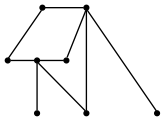
\includegraphics[width=2cm]{graph.png}
  \end{figure}
  When $\mathcal{I}$ is a family of forests, such as: \\
  \begin{figure}
   \centering
   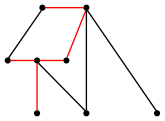
\includegraphics[width=2cm]{graph1.png}
   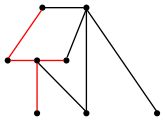
\includegraphics[width=2cm]{graph2.png}
   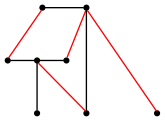
\includegraphics[width=2cm]{graph3.png}
   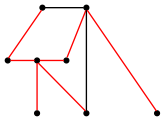
\includegraphics[width=2cm]{graph4.png}
   \;etc...
  \end{figure}

  Then $\mathcal{I}$ satisfies (1), (2), (3).
 \end{exampleblock}
\end{frame}

\section{Progress}
\begin{frame}{ON DISJOINT COMMON BASES IN TWO MATROIDS}
 \begin{block}{problem 1}
  Let $M_1 = (S, \mathcal{I}_1)$ and $M_2 = (S, \mathcal{I}_2)$ be matroids on the ground set $S$, where $\mathcal{I}_1$ and $\mathcal{I}_2$ are the respective families of independent sets. A set $B \subseteqq S$ that is both a base of $M_1$ and $M_2$ is called a common base. The problem is to decide whether $S$ can be partitioned into common bases.
 \end{block}
 \begin{figure}
  \centering
  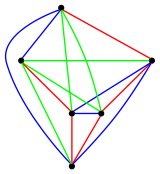
\includegraphics[width=2cm]{partitioned-graph.png}
  \caption{partitioned into bases}
 \end{figure}
\end{frame}

\begin{frame}{ON DISJOINT COMMON BASES IN TWO MATROIDS}
 \begin{alertblock}{conjecture 2 (Rota's conjecture)}
  Let $M = (T, \mathcal{I})$ be a matroid of rank $n$. Let $A_1 , ..., A_n$ be a partition of $T$ into bases of $M$. Then there are disjoint bases $B_1 , ..., B_n$ such that $|A_i \cap B_j| = 1$ for every $i = 1, ..., n$ and $j = 1, ..., n$.
 \end{alertblock}
 Next conjecture is the generalization of Rota's conjecture:
 \begin{alertblock}{conjecture 3 (Chow's conjecture)}
  Let $M = (T, \mathcal{I})$ be a matroid of rank $n$ with the property that $T$ can be partitioned into $b$ bases where $3 \leq b \leq n$. Let $I_1, ..., I_n \in \mathcal{I}$ be disjoint independent sets, each size at most $b$. Then there exists a partition of $T$ into sets $A_1, ..., A_n$ such that $I_i \subseteqq A_i$ and $|A_i| = b$ for every $i = 1, ..., n$, and there exist disjoint bases $B_1, ..., B_b$ such that $|A_i \cap B_j| = 1$ for every $i = 1, ..., n$ and $j = 1, ..., b$.
 \end{alertblock}
\end{frame}

\begin{frame}{ON DISJOINT COMMON BASES IN TWO MATROIDS}
 \begin{block}{theorem 4}
  Problem 1 can be solved in polynomial time if and only if this is under the additional assumption that one of the matroids is a direct sum of uniform matroids.
 \end{block}
 \begin{block}{definition}
  Let $M_1 = (E_1, \mathcal{I}_1),\; M_2 = (E_2, \mathcal{I}_2)$ be matroids where $E_1 , E_2 \neq \emptyset , E_1 \cap E_2 = \emptyset$.\\
  M is called a \alert{direct sum} of 2 matroids, $M_1$ and $M_2$ when:
  \begin{align*}
   M = (E_1 \cup E_2 ,\; &\mathcal{I}_1 \oplus \mathcal{I}_2) \\
   where\; &\mathcal{I}_1 \oplus \mathcal{I}_2 = \{X_1 \cup X_2\; |\; X_1 \in \mathcal{I}_1, X_2 \in \mathcal{I}_2\}
  \end{align*}
 \end{block}
\end{frame}

\begin{frame}
 \begin{exampleblock}{uniform matroid}
  Let $U = (S, \mathcal{I})$ be a matroid where $\mathcal{I} \in 2^S$ satisfies:
  \begin{align*}
   \mathcal{I} = \{I\;|\;|I| \leq k\}
  \end{align*}
  Then $U$ is a matroid of rank $k$. This $U$ is called a \alert{uniform matroid}.
 \end{exampleblock}
\end{frame}

\begin{frame}
 \begin{block}{claim 5}
  Conjecture 3 is false for every b such that $2 \leq b \leq \frac{n}{3}$.
 \end{block}
 \begin{block}{corollary 6}
  Problem 1 can be solved in polynomial time if and only if this is true under the additional assumption that $M_2$ is a direct sum of uniform matroids whose blocks are each independent in $M_1$.
 \end{block}
\end{frame}

\section{Next step}
\begin{frame}{next month}
 Yet these methods show that Chow's conjecture is false when $3 \leq b \leq \frac{n}{3}$, Rota's conjecture is still alive since it's Chow's conjecture in the case of $b = n$. There's still room for research about Chow's conjecture. \\
 Also, computational complexity of problem 1 is still open. This paper gives neccesary and sufficient condition to solve problem 1 in polynomial time only when problem 1 can be solved. It's yet to be discovered exactly when problem 1 can be solved. \\
 What I'm going to do next month is to think about these problems.
\end{frame}

\begin{frame}
 \begin{center}
  Thank you for your attention.
 \end{center}
\end{frame}
\end{document}